\documentclass[../main.tex]{subfiles}


\begin{document}
	\section{Kam dál?}
	O ovládání robota se v této učebnici více nedozvíte. Její zbytek je věnovaný tomu, kam se vydat, pokud máte zájem dál rozvíjet vzdělání v oboru robotiky a informatiky.

	\subsection{Robotické soutěže}
	Firma VEX pořádá \href{https://www.vexrobotics.com/competition?___store=vexroboticseu&___from_store=vexrobotics}{několik soutěží} (pro své různé stavebnice), převážně pro studenty středních škol, které jsou zaměřené na stavění a programování robota. Většinou je potřeba robota naprogramovat, aby plnil (autonomně i ovládaný hráčem) různé úkoly.

	Je nemalá šance, že někde ve vašem okolí už existuje tým robotiky, který se této nebo jiné soutěži věnuje. V případě zájmu o účast v nějaké robotické soutěži ho rozhodně doporučuji kontaktovat -- lidí nadšených do robotiky není nikdy dost.

	Pokud žádný tým v okolí neexistuje, tak je vždy možné (byť pracnější a nákladnější) ho založit. 

	\subsection{Python}
	Python je jeden z nejpopulárnějších jazyků světa a je využívaný v nesčetné řadě oborů (statistika, matematika, vývoj aplikací, robotika). Možná si to neuvědomujete, ale v Pythonu jsme vlastně programovali celou dobu -- Blocky je pouze nadstavba, která je před spuštěním přeložena do Pythonu. Stačí stisknout \centerimage{\baselineskip}{Images/ui/generated-code.png}, k nalezení pod ovládací částí.

	Následující Blocky program:

	\begin{figure}[h!]
		\centering
		\begin{minipage}{0.50\textwidth}
			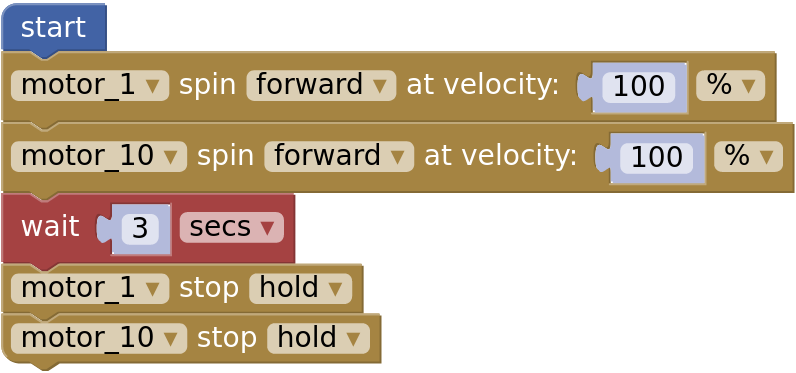
\includegraphics[width=\linewidth]{Images/06/program.png}
		\end{minipage}
	\end{figure}

	se pro příklad přeloží na následující Python program:

	\begin{figure}[h!]
		\centering
		\begin{minted}{python}
			import vex
			import drivetrain
			import smartdrive
			import sys

			#region config
			brain    = vex.Brain()
			motor_1  = vex.Motor(vex.Ports.PORT1, vex.GearSetting.RATIO18_1, False)
			motor_10 = vex.Motor(vex.Ports.PORT10, vex.GearSetting.RATIO18_1, False)
			#endregion config

			# main thread
			motor_1.spin(vex.FORWARD, 100, vex.PERCENT)
			motor_10.spin(vex.FORWARD, 100, vex.PERCENT)
			vex.wait(3,vex.SECONDS)
			motor_1.stop(vex.BrakeType.HOLD)
			motor_10.stop(vex.BrakeType.HOLD)
		\end{minted}
	\end{figure}

	Ke studiu Pythonu existuje řada online zdrojů. Jeden, vhodný pro začátečníky, je např. \href{https://coherentpdf.com/python/pythonfromtheverybeginning.html}{Python from the very beginning}. Python představuje od úplných základů a obsahuje řadu cvičení (i s nápovědami a řešeními), díky kterým se z něho učí příjemně.

	Pro rychlý přehled důležitějších konceptů a další nápady na příklady (a jejich řešení) si doporučuji projet \href{https://slama.dev/programovani-je-hra/}{poznámky ke kurzu Programování je hra}, který jsem v roce 2020/2021 organizoval.

	Mimo to je obecně dobrý nápad zkusit vaše Blocky programy překládat od Pythonu -- pokud chápete, co dělá daný Blocky program, tak je jednodušší rozumět i stejnému programu napsanému v Pythonu.

	\subsection{Algoritmy a datové struktury}
	Pokud byste raději chtěli zkusit řešit příklady spíše teoreticky, tak jedno ze skvělých míst je \href{http://ksp.mff.cuni.cz/}{Korespondenční Seminář z Programování} (především \href{http://ksp.mff.cuni.cz/z/}{kategorie Z}). Jedná se o korespondenční seminář plný bezva lidí (a taky mě), kteří jsou nadšení do informatiky.

	Podrobnější (ale na čtení znatelně obtížnější) je \href{http://pruvodce.ucw.cz/}{Průvodce labyrintem algoritmů}, který rozebírá řadu běžně používaných algoritmů a datových struktur a měla by spíše sloužit jako reference než jako učebnice.

\end{document}
